\section{Univariate UQ}
In this section we limit ourselves to the analysis of the UQ algorithm as it applies to univariate versions of the deterministic solvers.  This gives a baseline before approaching multivariate inputs in their variety.

\subsection{Polynomial Solver: $f(x)$}
The purpose of the polynomial solver is to demonstrate convergence on an analytic mean, variance, and pdf for both Monte Carlo and PCESC methods.  We consider two cases.  In the first, $x$ is distributed uniformly as $x\sim\mathcal{U}(3,7)$.  In the second, $x$ is distributed normally as $x\sim\mathcal{N}(5,4)$.  The expected analytic moments are given in Table \ref{tab:poly uni mom}.
\begin{table}[H]
\centering
\begin{tabular}{c|c|c}
Distribution & $m_1$ & var \\ \hline
$\mathcal{U}(3,7)$ & 11 & 79/3\\
$\mathcal{N}(5,4)$ & 11 & 16
\end{tabular}
\caption{Analytic Moments for Univariate Polynomial Solver}
\label{tab:poly uni mom}
\end{table}
Because this case expands a first-order polynomial in polynomials, it can be exactly replicated with a first-order expansion.  Table \ref{tab:poly uni res} shows the Monte Carlo and PCESC statistics.  The solution PDFs are in Fig. \ref{fig:poly uni res}.

\begin{table}[H]
\begin{center}
\begin{tabular}{c|c c|l l}
Distr. & UQ & runs$|$order & mean & variance \\ \hline
Uniform & MC & $1\times10^7$ & 10.999555712 & 5.3374535046 \\
 & SC & 2 & 11.0 & 5.33333333333 \\ \hline
Normal & MC & $1\times10^7$ & 11.0000448162 & 15.9892244775 \\
 & SC & 2 & 11 & 16 
\end{tabular}
\end{center}
\caption{Polynomial Solver, Univariate Statistics}
\label{tab:poly uni res}
\end{table}

\begin{figure}[H]
\centering
  \begin{subfigure}[b]{0.4\textwidth}
   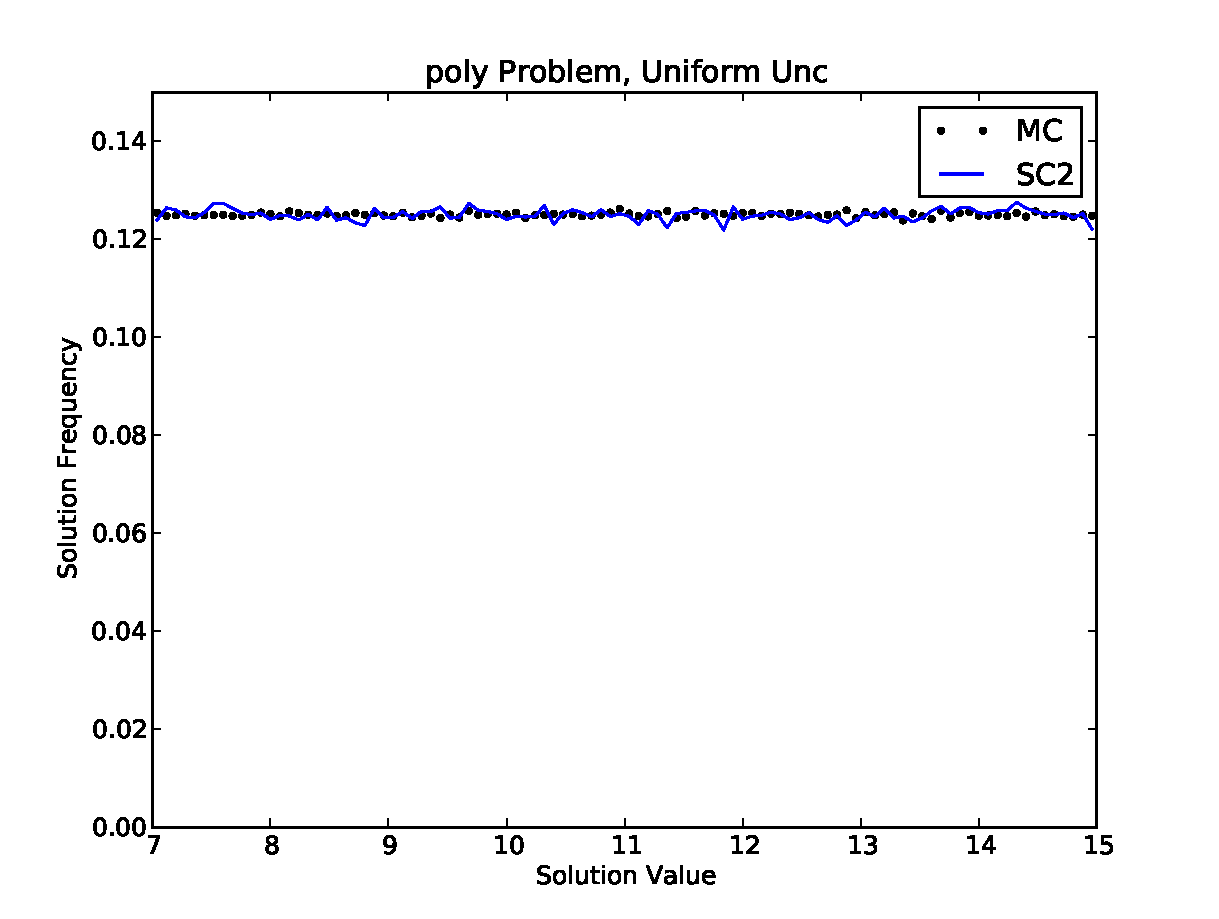
\includegraphics[width=\textwidth]{../graphics/poly_uniform_pdfs}
   \caption{Uniform}
      \label{fig:poly uni}
  \end{subfigure}
  \begin{subfigure}[b]{0.4\textwidth}
   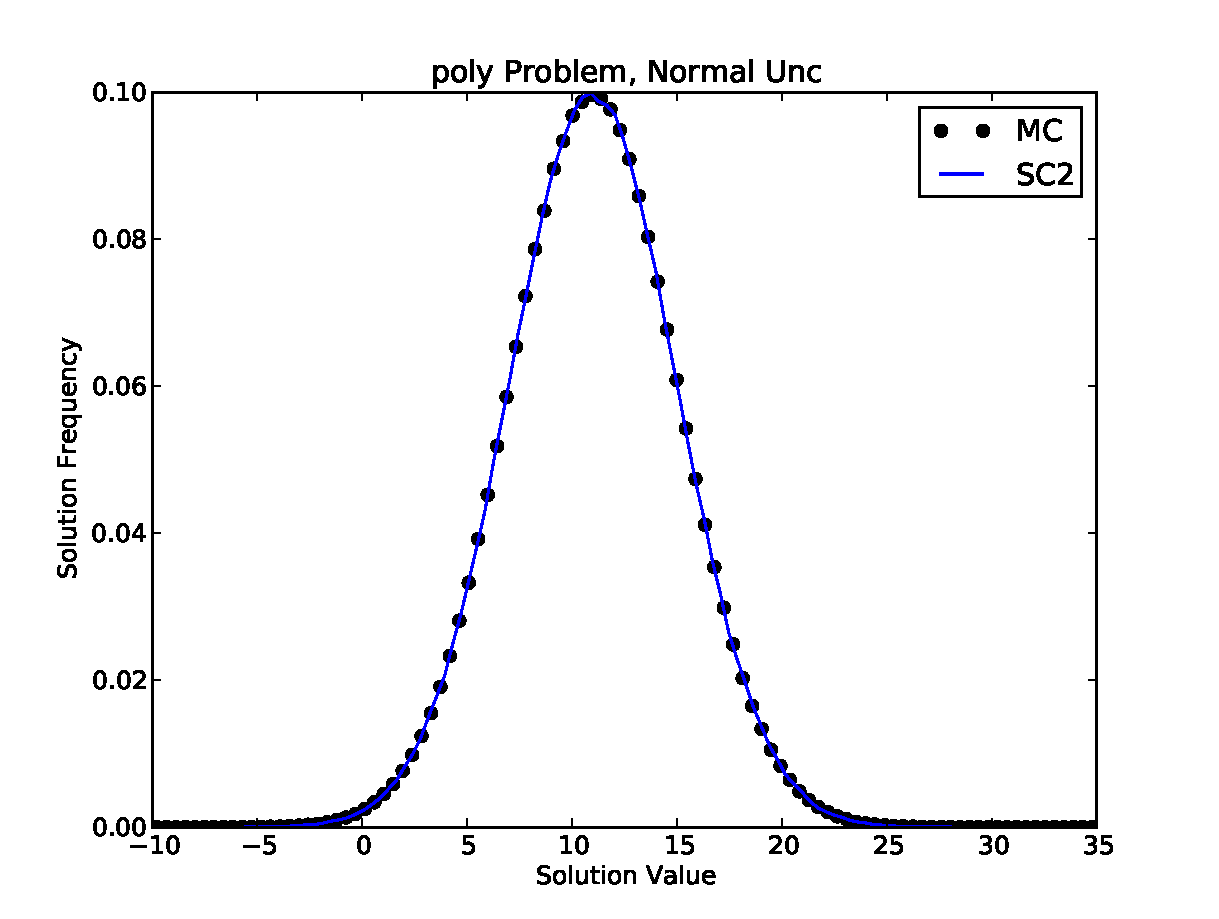
\includegraphics[width=\textwidth]{../graphics/poly_normal_pdfs}
   \caption{Normal}
      \label{fig:poly norm}
  \end{subfigure}
  \caption{Univariate Polynomial Solver PDFs}
  \label{fig:poly uni res}
\end{figure}

\subsection{Source Solver: $\phi=\phi\qty(S,D,x,\Sigma_a)$}
For the univariate case, we introduce uncertainty in the absorption cross section $\Sigma_a$.  We consider two cases: first, when $\Sigma_a\sim\mathcal{U}(0.5,1)$; second, when $\Sigma_a\sim\mathcal{N}(0.75,0.0225)$.  The other parameters are
\begin{align}
S &= 1.0 \text{ n/cm}^2\text{/s},\\
D &= 0.5 \text{ /cm},\\
x &= 2.0 \text{ cm}.
\end{align}
We consider several increasing levels of polynomial expansion and the convergence onto the Monte Carlo solution.  The results are in Table \ref{tab: source uni res}.  The solution PDFs are in Fig. \ref{fig:source uni res}.

\begin{table}[H]
\begin{center}
\begin{tabular}{c|c c|l l}
Distr. & UQ & runs$|$order & mean & variance \\ \hline
Uniform & MC & $1\times10^6$ & 1.26069628111 &  0.0632432419713 \\
 & SC & 2 & 1.25774207229 & 0.0495341371244 \\
 & SC & 4 & 1.26064320417 & 0.0604388749588 \\
 & SC & 8 & 1.26108375978 & 0.0637370898233\\
 & SC & 16 & 1.26112339681 & 0.0639754882641 \\ \hline
Normal & MC & $1\times10^6$ & 1.24922240195 & 0.0488719424418 \\
&SC & 2 & 1.2547221522 & 0  \\
&SC & 4 & 1.25569029702 & 0.049198975952  \\
&SC & 8 & 1.25569096924 & 0.0492316191443 \\
&SC & 16 & 1.25569096924 & 0.0492316191611
\end{tabular}
\end{center}
\caption{Source Solver, Univariate Statistics}
\label{tab: source uni res}
\end{table}

\begin{figure}[h]
\centering
  \begin{subfigure}[b]{0.45 \textwidth}
   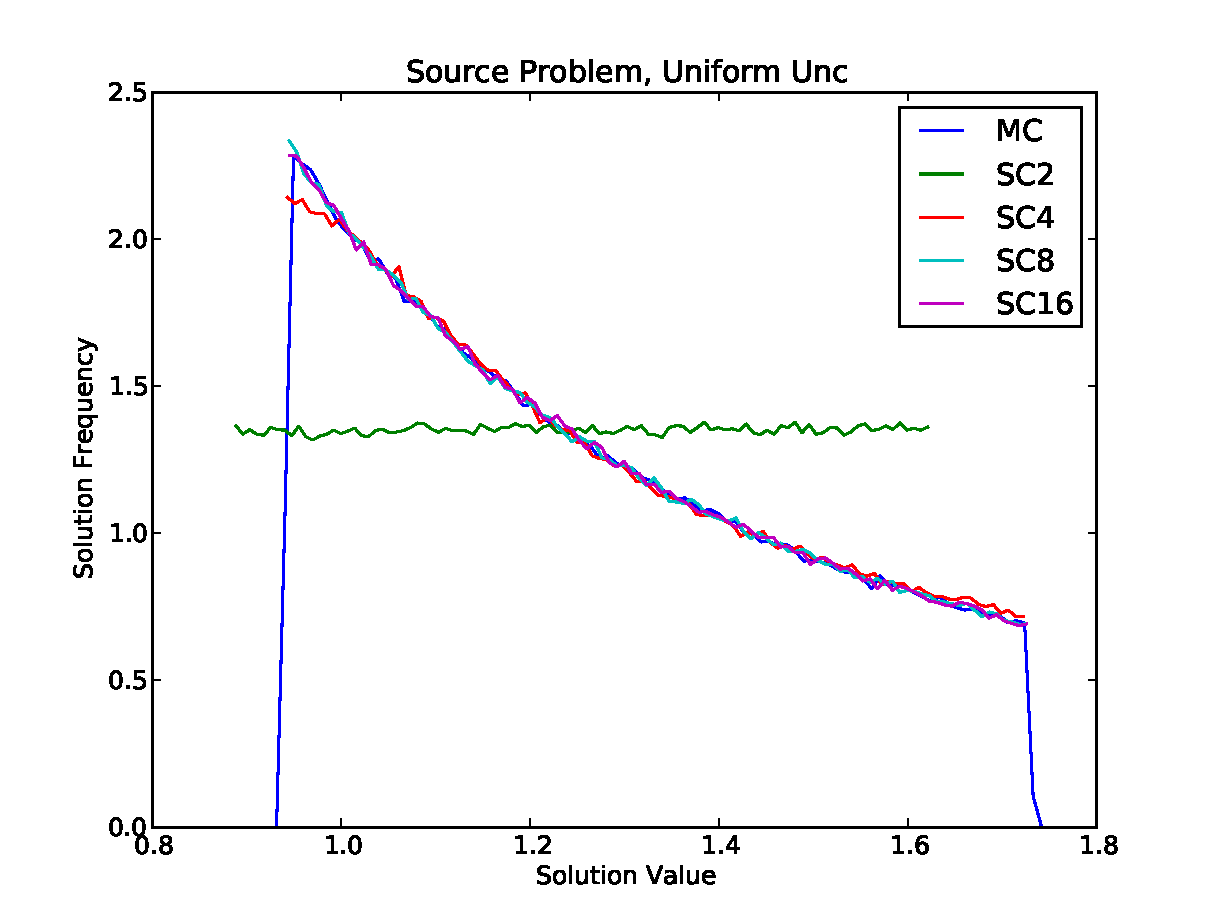
\includegraphics[width=\textwidth]{../graphics/source_uniform_pdfs}
   \caption{Uniform}
      \label{uni}
  \end{subfigure}
  \begin{subfigure}[b]{0.45\textwidth}
   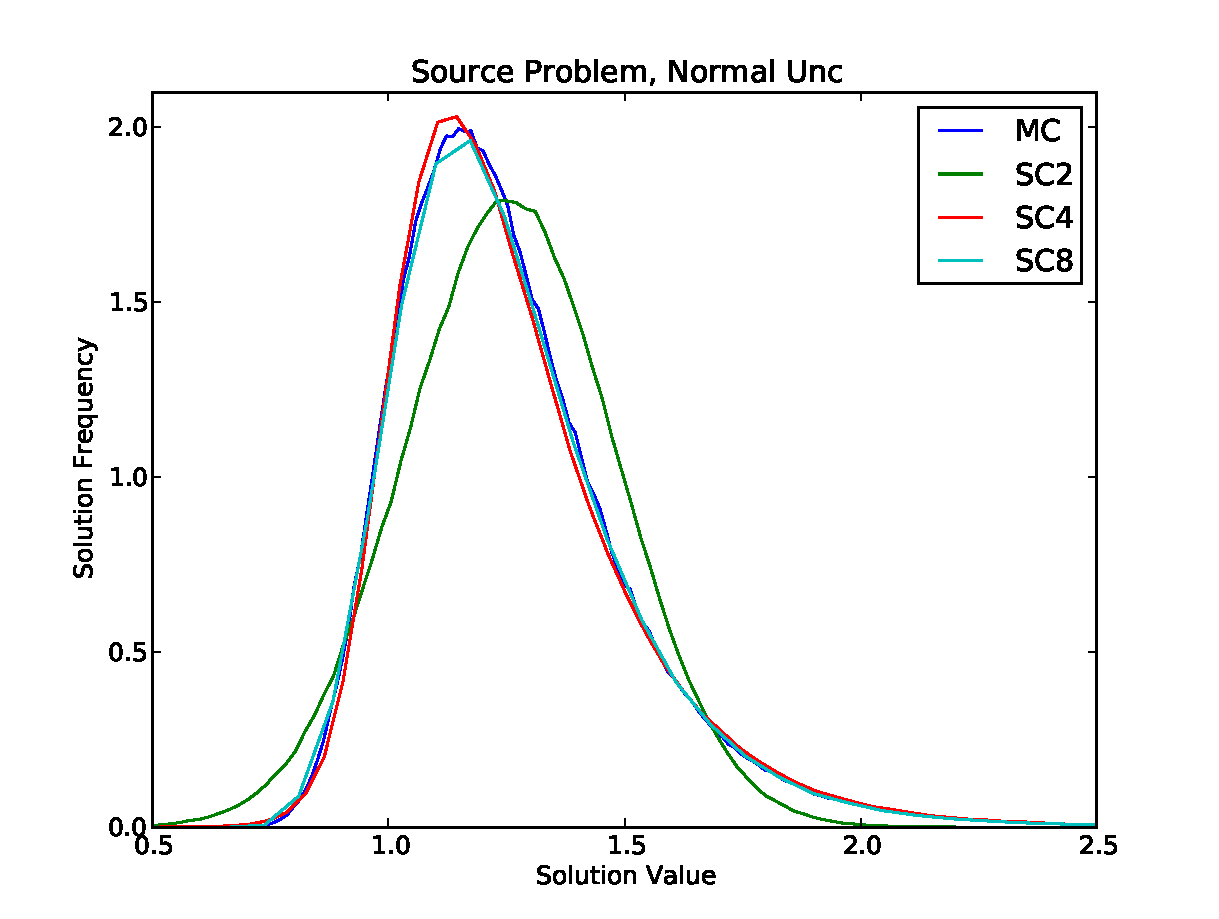
\includegraphics[width=\textwidth]{../graphics/source_normal_pdfs}
   \caption{Normal}
      \label{norm}
  \end{subfigure}
\caption{Univariate Source Solver PDFs}
\label{fig:source uni res}
\end{figure}

\subsection{1D Diffusion Solver: $k=k\qty(D_g,\Sigma_{g,c},\Sigma_{g'\to g,s},\Sigma_{g,f},\nu_g)$}
For the univariate case, we introduce uncertainty in the neutron capture cross section of the second energy group $\Sigma_{2,c}$.   We consider three cases, $\Sigma_{2,c}$ distributed normally in each.  We choose a different mean for each distribution.  Each mean corresponds to a different reactivity state: subcritical, critical, and supercritical ($k=(0.9,1.0,1.1)$).  The three distributions are respectively $\Sigma_{2,c}\sim\qty(\mathcal{N}(0.055969,0.1),\mathcal{N}(0.04438,0.1),\mathcal{N}(0.035181,0.1))$.  We also restrict Monte Carlo sampling of the uncertain parameter to three standard deviations around the mean, effectively creating a truncated normal distribution.  For this reason, the mean and variance of the Monte Carlo sampling do not converge on the analytic values.  The results are shown in Table \ref{tab: 1d uni res}.  The solution PDFs are shown in Fig. \ref{fig:1d uni res}.
\begin{table}[H]
\begin{center}
\begin{tabular}{c|c c|l l}
Type & UQ & runs$|$order & mean & variance \\ \hline
Subcritical & MC & $1\times10^6$ & 0.907699673282 & 0.00632790358771 \\
&SC & 2 & 0.907653521565 & 0.00595095987773 \\
&SC & 4 & 0.907813174929 & 0.00633526057266\\
&SC & 8 & 0.907813389468 & 0.00633649118503 \\
&SC & 16 & 0.907813389471 & 0.00633649126226 \\ \hline
Critical &MC & $1\times10^6$ & 1.01144778738 & 0.0105716289269   \\
&SC & 2 & 1.01107577584 & 0.00974910361412  \\
&SC & 4 & 1.0113755955 & 0.0105739848126 \\
&SC & 8 & 1.01137628238 & 0.0105785232446 \\
&SC & 16 & 1.01137628243 & 0.0105785241745 \\ \hline
Supercritical & MC & $1\times10^6$ & 1.11593980088 & 0.0168503796482 \\
&SC & 2 & 1.11537873568 & 0.0151539223359 \\
&SC & 4 & 1.11590698755 & 0.016795821961\\
&SC & 8 & 1.11590896034 & 0.0168106966474 \\
&SC & 16 & 1.11590896088 & 0.0168107061554
\end{tabular}
\end{center}
\caption{1D Solver, Univariate Statistics}
\label{tab: 1d uni res}
\end{table}

\begin{figure}[h!]
\centering
   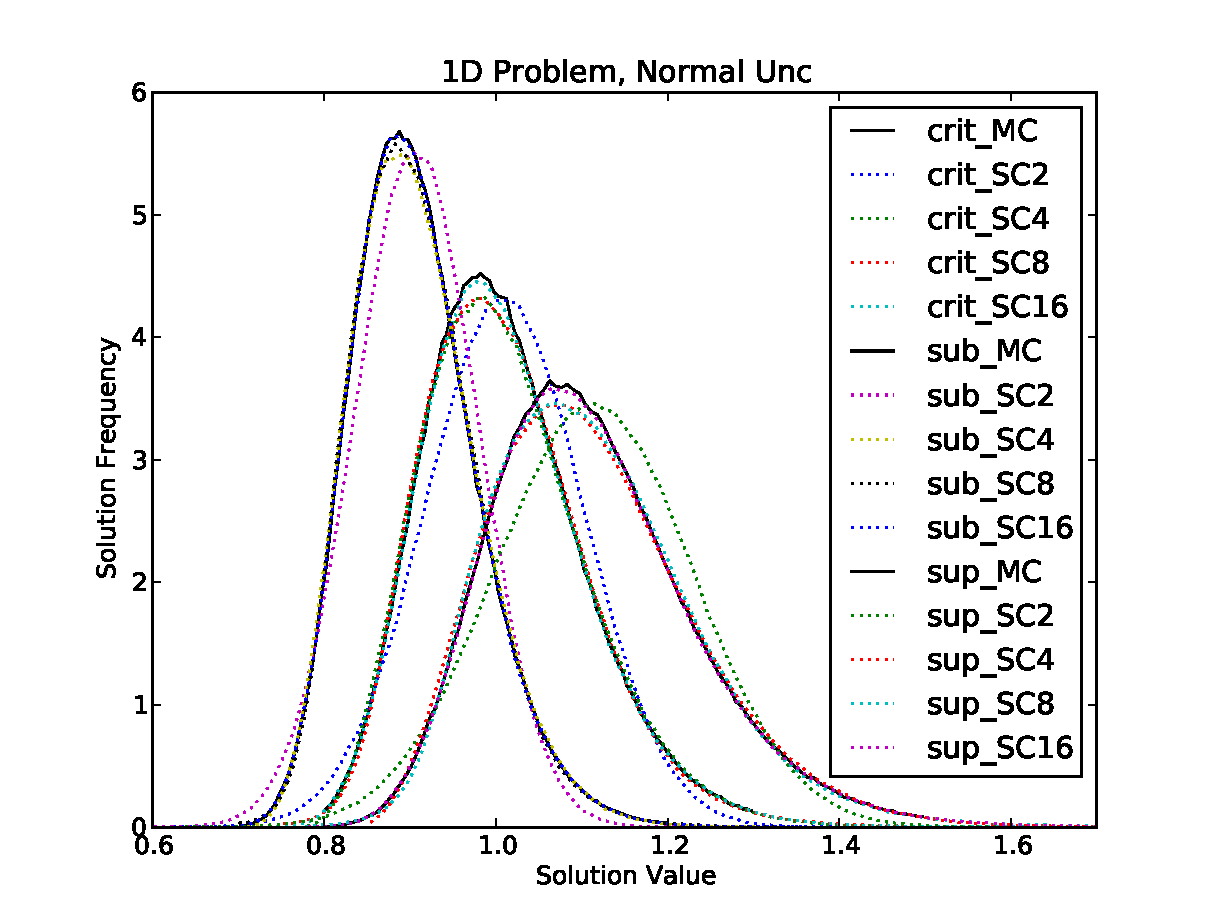
\includegraphics[width=.75\textwidth]{../graphics/1dall_normal_pdfs}
   \caption{Univariate 1D Solver PDFs}
   \label{fig:1d uni res}
\end{figure}


\newpage
\subsection{Quarter Core Solver: $k=k\qty(D_g^{(R)},\xs{g,c}{R},\xs{g'\to g,s}{R},\xs{g,f}{R},\nu_g^{(R)})$}
The original benchmark parameters before introducing uncertainty are in Table \ref{tab:coremats}.
\begin{figure}[H]
\centering
   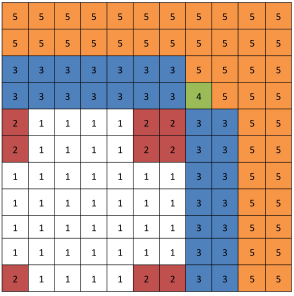
\includegraphics[width=0.4\textwidth]{../graphics/core}
   \caption{Quarter Core Map}
\end{figure}
\begin{table}[H]
\centering
\begin{tabular}{c c | c c c c}
Material (R)& Group & $D_g^{(R)}$ & $\xs{g,c}{R}$ & $\nu\xs{g,f}{R}$ & $\xs{1\to2,s}{R}$ \\ \hline
1 & 1 & 1.255    & 4.602e-3 & 4.602e-3 & 2.533e-2 \\
  & 2 & 2.11e-1  & 5.540e-2 & 1.091e-1 & \\ \hline
2 & 1 & 1.268    & 4.609e-3 & 4.609e-3 & 2.767e-2 \\
  & 2 & 1.902e-1 & 8.675e-2 & 8.675e-2 & \\ \hline
3 & 1 & 1.259    & 6.083e-3 & 4.663e-3 & 2.617e-2 \\
  & 2 & 2.091e-1 & 4.142e-2 & 1.021e-1 & \\ \hline
4 & 1 & 1.259    & 4.663e-3 & 4.663e-3 & 2.617e-2 \\
  & 2 & 2.091e-1 & 3.131e-2 & 1.021e-1 & \\ \hline
5 & 1 & 1.257    & 6.034e-4  & 0 & 4.754e-2 \\
  & 2 & 1.592e-1 & 1.911e-2  & 0 & 
\end{tabular}
\caption{Material Properties for Core}
\label{tab:coremats}
\end{table}
Similar to the one-dimensional problem, we introduce uncertainty in the low-energy capture cross section, in this case only in Material 1 $\qty(\xs{2,c}{1})$, which makes up the majority of the core.  We consider two distributions, $\xs{2,c}{1}\sim\qty(\mathcal{U}(0.0454,0.0654),\mathcal{N}(0.0554,0.01^2))$.  Because of the nonlinear dependence of the solution on the input parameter, we use order 32 Gauss quadrature to obtain all the polynomial expansion coefficients, instead of scaling them with the total expansion order.  The Monte Carlo sampling algorithm rejects samples outside three standard deviations, causing discrepancy in the mean and variance.
\begin{table}[H]
\begin{center}
\begin{tabular}{c|c c|l l}
Type & UQ & runs$|$order & mean & variance \\ \hline
Uniform &MC & $1\times10^6$ & 1.00406413634 & 0.000446173081079 \\
&SC & 2  & 1.00416405471 & 0.000375112851817 \\
&SC & 4  & 1.00416405471 & 0.000390962150246 \\
&SC & 8  & 1.00416405471 & 0.000406864600682 \\
&SC & 16 & 1.00416405471 & 0.000421349517322 \\
&SC & 32 & 1.00416405471 & 0.000425027572716 \\ \hline
Normal &MC & $1\times10^6$ & 1.01333702129 & 0.00160652595587 \\
&SC & 2  & 1.01643813464 & 0.00138703446968 \\
&SC & 4  & 1.01643813464 & 0.00184314998697 \\
&SC & 8  & 1.01643813464 & 0.00184690058216 \\
&SC & 16 & 1.01643813464 & 0.00184724103523 \\
&SC & 32 & 1.01643813464 & 0.00184726152781
\end{tabular}
\end{center}
\caption{Quarter Core Solver, Univariate Statistics}
\label{tab: 2d uni res}
\end{table}

%\begin{figure}[h]
%\centering
%  \begin{subfigure}[b]{0.45 \textwidth}
%   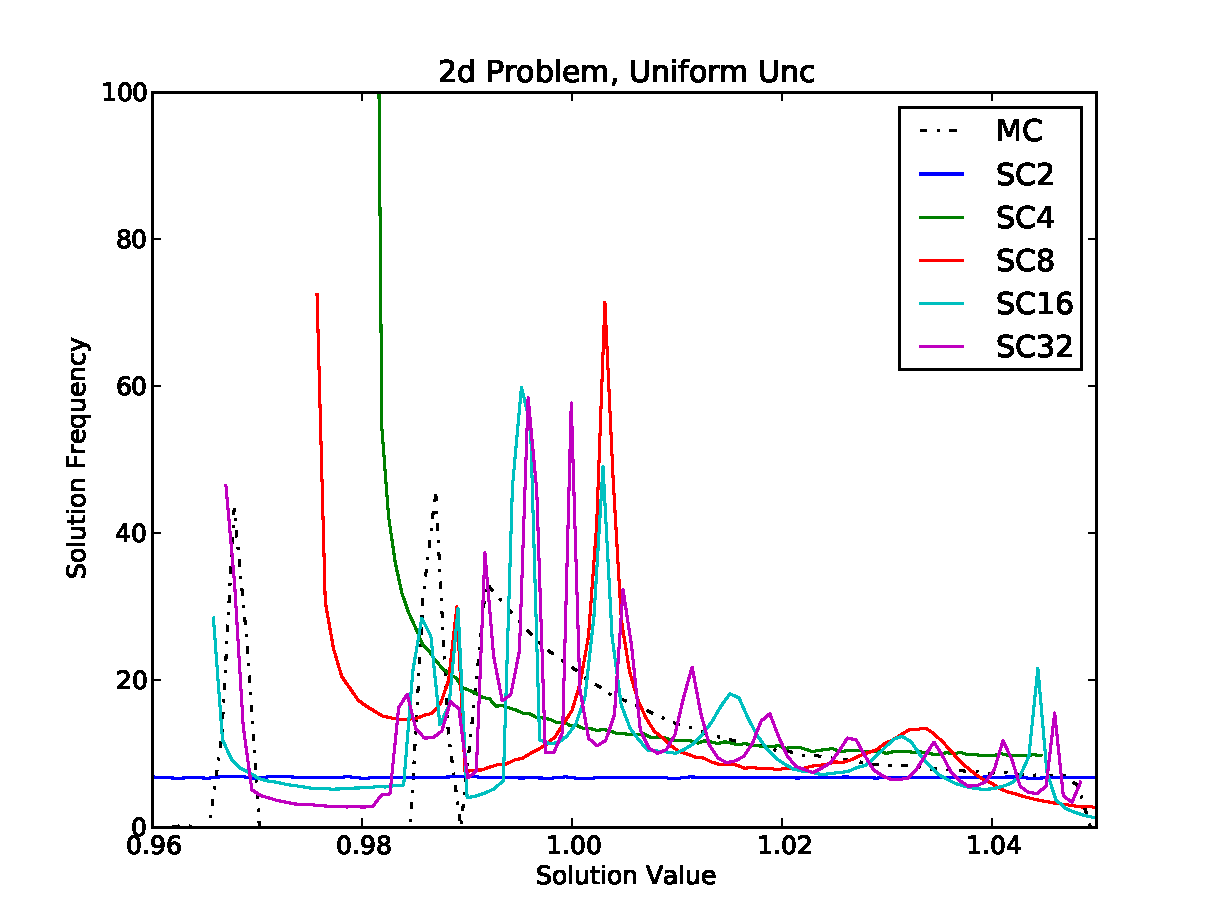
\includegraphics[width=\textwidth]{../graphics/2d_uniform_pdfs}
%   \caption{Uniform}
%      \label{uni}
%  \end{subfigure}
%  \begin{subfigure}[b]{0.45\textwidth}
%   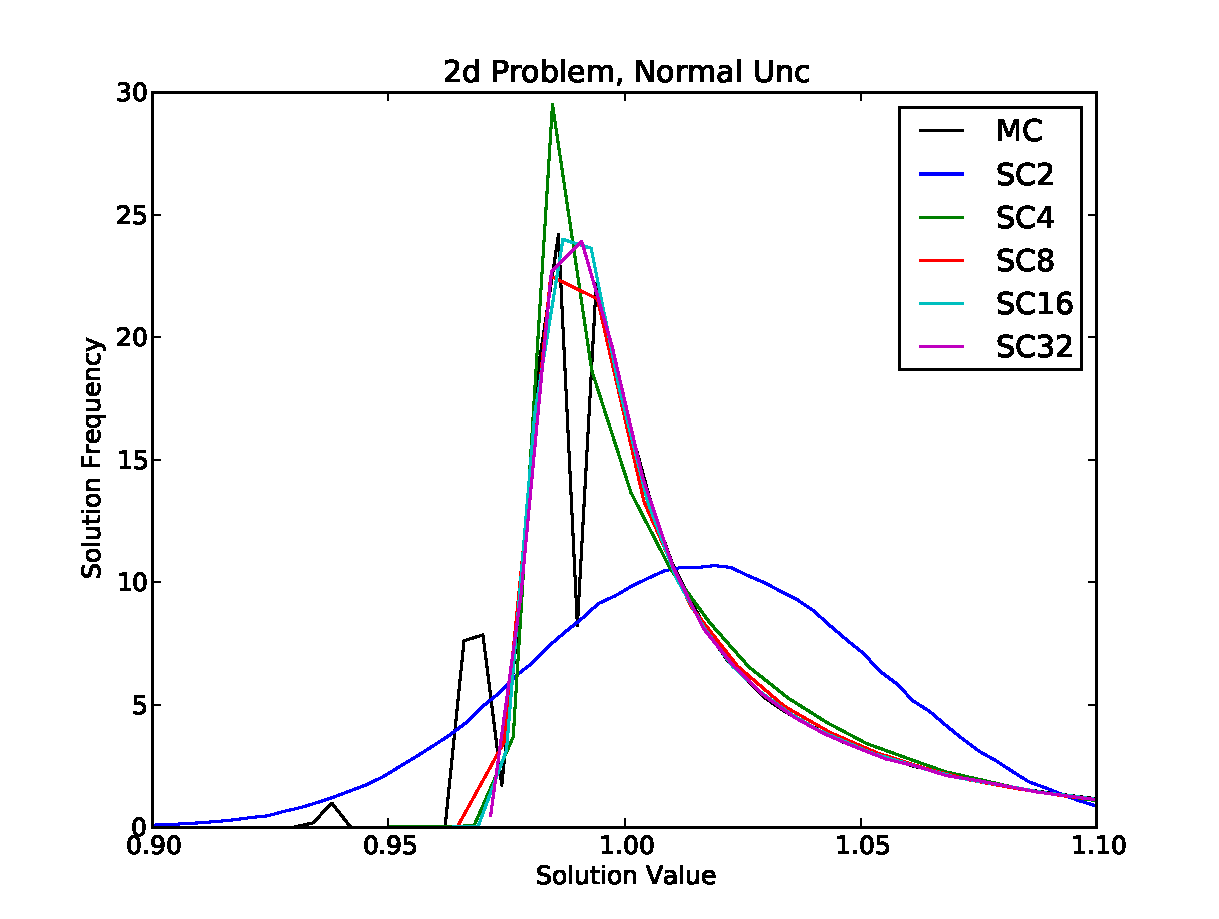
\includegraphics[width=\textwidth]{../graphics/2d_normal_pdfs}
%   \caption{Normal}
%      \label{norm}
%  \end{subfigure}
%\caption{Univariate Quarter Core Solver PDFs}
%\label{fig:source uni res}
%\end{figure}
\begin{figure}[H]
\centering
   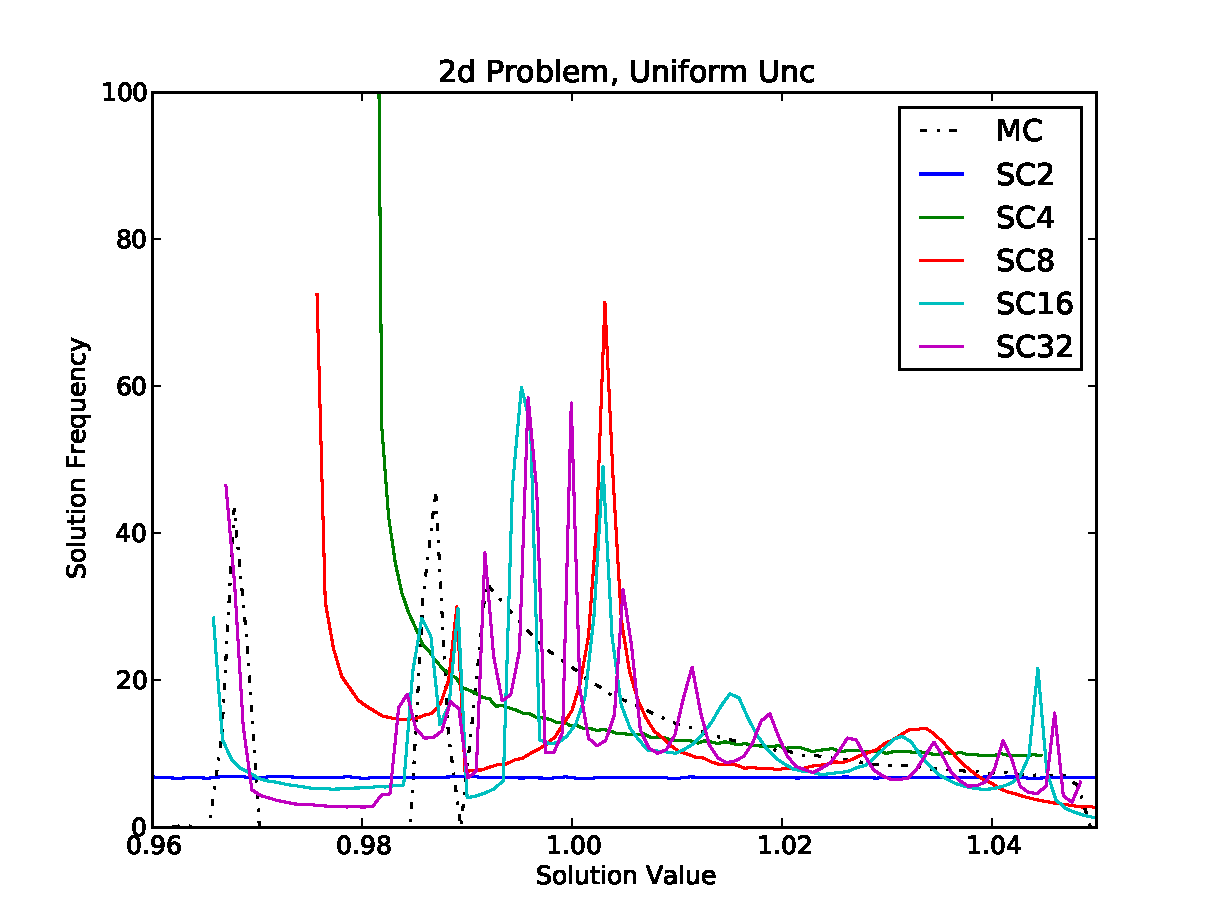
\includegraphics[width=0.7\textwidth]{../graphics/2d_uniform_pdfs}
   \caption{Uniform Univariate Quarter Core Solver PDFs}
   \label{fig:2dcrit uni}
\end{figure}
\begin{figure}[H]
\centering
   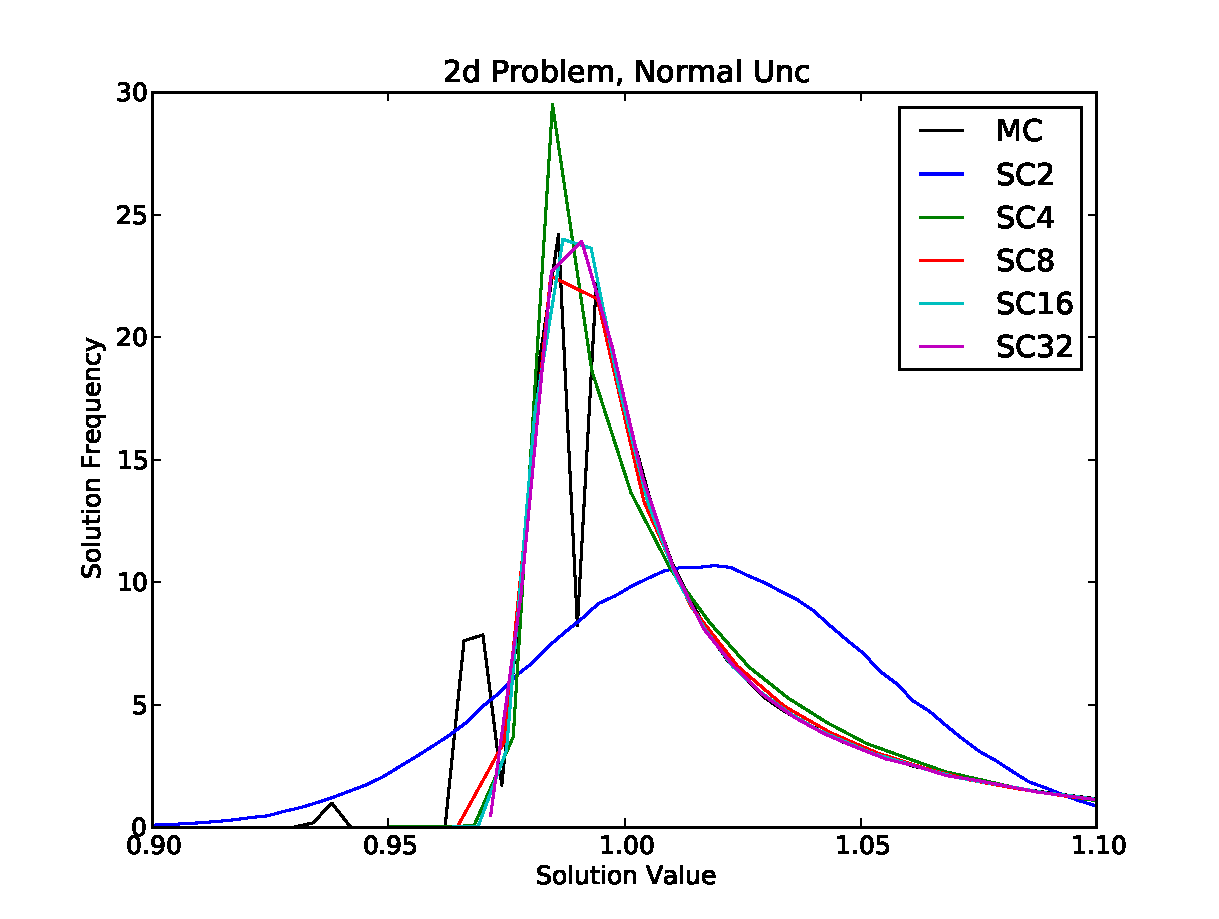
\includegraphics[width=0.7\textwidth]{../graphics/2d_normal_pdfs}
   \caption{Normal Univariate Quarter Core Solver PDFs}
   \label{fig:2dcrit}
\end{figure}
